%	$Id$
% Internal documentation for slide modeling in grdseamount
% Paul Wessel, November 16, 2016.
\documentclass[12pt,letterpaper,margin=0.5in]{report}
\usepackage{times}
\usepackage{graphicx}
\usepackage{breqn}
\usepackage[margin=0.5in]{geometry}
\usepackage{lscape}
\textheight = 9 in
\topmargin = -1 in
\begin{document}

\section{Model landslides in grdseamount}

\begin{figure}[h!]
  \centering
  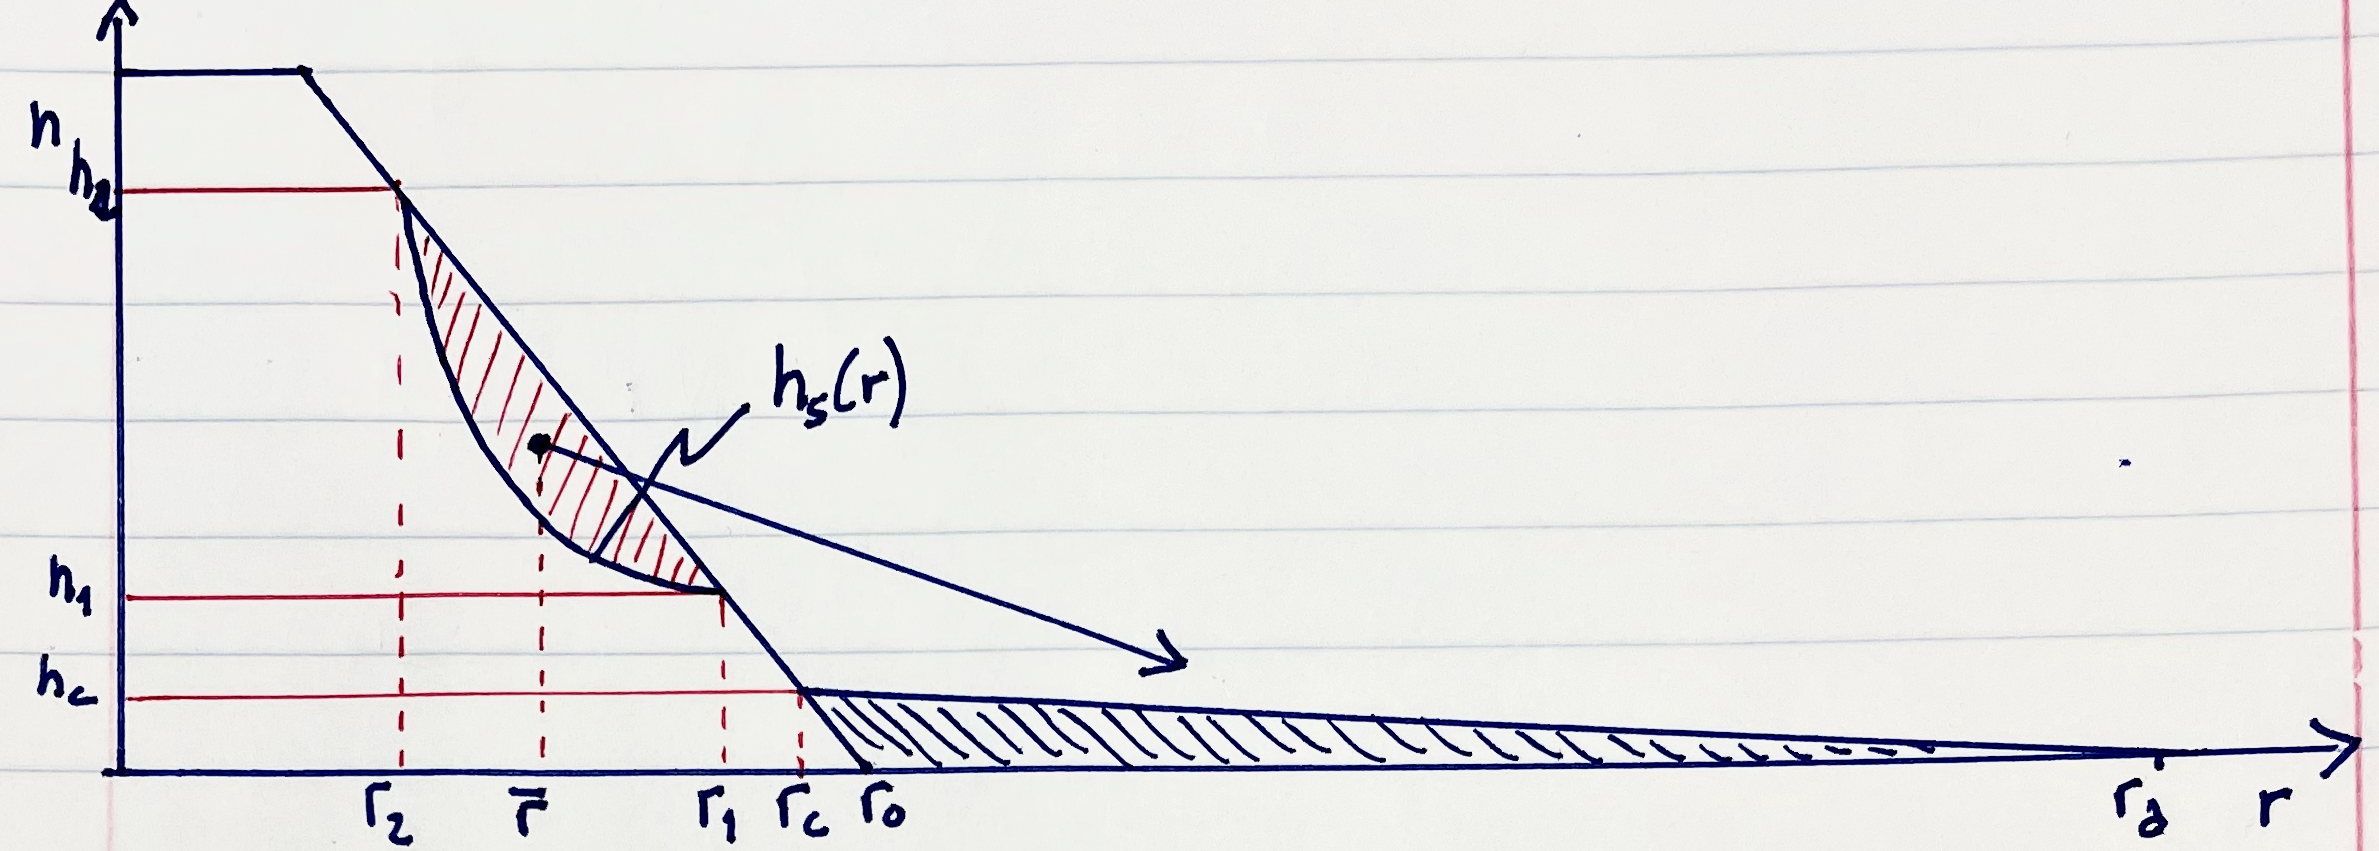
\includegraphics[width=5in]{slides_fig1.png}
  \caption{Geometry for an \emph{ad hoc} landslide approximation in \texttt{grdseamount}.  The slide material (red hachured area)
  will be deposited at the toe of the seamount (blue hachured area) reaching up to a height of $h_c$ and linearly
  tapering to zero at a distal point $r_d$. Note that $h_2 > h_1$ while $r_1 > r_2$.}
  \label{slides_fig1}
\end{figure}

These notes expands the work of {\it J. Smith and Wessel} (2000) on approximating large landslides off seamounts
for the purpose of studying the isostatic consequences.  I refer to Figure~\ref{slides_fig1}.  The equation for the
cross-sectional shape of the slide for the radial range $r_2$ to $r_1$ is given by a single equation:
\begin{equation}
h_s(r) = h_1 + \Delta h \cdot q(u),
\end{equation}
where $\Delta h = h_2 - h_1$ is the \emph{height} range of the rupture surface and $q(u)$ is the normalized shape curve of the slide,
\begin{equation}
q(u) = u_0 \left (\frac{1 + u_0}{u + u_0} - 1 \right ),
\end{equation}
which is a hyperbolic curve. We use the tuning parameter $u_0$ to carve more or less deeply into the seamount core,
which is an improvement upon the fixed scheme in {\it J. Smith and Wessel} (2000).
Here, $u$ is the normalized distance from $r_2$ to $r_1$, given by
\begin{equation}
u = \frac{r-r_2}{r_1 - r_2} = \frac{r-r_2}{\Delta r},
\end{equation}
where $\Delta r$ is the \emph{radial} range of the slide.
Figure~\ref{slides_fig2} shows typical shapes of $q(u)$ for values of $u_0$.
\begin{figure}[h!]
  \centering
  \includegraphics[width=5in]{slides_fig2.png}
  \caption{A variety of slide shapes are possible by varying $u_0$.  The slide area for a conical seamount would be the area
  between the flank (dashed line) and the selected curve.}
  \label{slides_fig2}
\end{figure}

Depending on the shape of the seamount prior to the slide event (called $h(r)$, with $h_s(r) \le h(r)$), we will need to compute the various radii referred
to in Figure \ref{slides_fig1}, such as $r_1$, $r_2$, $r_c$, and $r_d$ from their corresponding heights $h_1$, $h_2$, $h_c$ and volume of slide.
The material removed by the land slide (red hachured area)
will be deposited at the base of the seamount (blue hachured area) up to the proximal height $h_c$.  We assume this deposit will have a linearly
decaying height, enabling us to compute the distal radius $r_d$ from the volume of the slide, $V_s$.  Clearly $V_s$ depends
on both $h(r)$ and $h_s(r)$.  We will compute this volume as $V_s = V_f - V_q$, where $V_f$ is the flank volume whose
trapezoidal (for a cone) crossection is delimited by the lines $r = r_2$, $h = 0$ and $h(r)$.  Its area $A_f$ and centroid $\bar{r}_f$ are computed once and
we then use Pappas' theorem to get the corresponding volume $V_f = 2 \pi \bar{r}_f A_f$.  For $V_s$ the upper limit is $h_s(r)$ instead of $h(r)$ so we can integrate
$h_s(r)$ for an analytical answer. First we get the area. To simplify we first only compute the upper part of the area, $A^u_s$ and later we add the pedestal area $A^l_s$ below $h_1$:
\begin{equation}
A^u_s = \int_{r_2}^{r_1} \Delta h q(u) dr = \Delta h \Delta r \int_0^1 q(u) du = \Delta h \Delta r u_0 \left [ (1 + u_0) \log \left (\frac{1 + u_0}{u_0} \right ) - 1 \right ].
\end{equation}
To use Pappas' theorem for computing the volume we need the radius to the centroid, which is obtained via
\begin{equation}
\bar{r}^u_s = \frac{\int_{r_2}^{r_1}q(u)rdr}{\int_{r_2}^{r_1}q(u)dr} = r_2 + \Delta r \bar{u}_s = r_2 + \Delta r \frac{\int_0^1q(u)udu}{\int_0^1 q(u)du}.
\end{equation}
This integral yields
\begin{equation}
\bar{u}^u_s = \frac{2(1 + u_0)\left [1 - u_0 \log \left ( \frac{1+u_0}{u_0} \right ) \right ] - 1}{(1 + u_0) \log \left (\frac{1 + u_0}{u_0} \right ) - 1}.
\end{equation}
The actual area under the $h_s(r)$ curve can then be written as
\begin{equation}
A_s = A^u_f + A^l_f = A^u_f + h_1 \Delta r.
\end{equation}
To compute the volume of the pedestal we also need its centroid radius:
\begin{equation}
\bar{r}^l_s = \frac{\int_{r_2}^{r_1} h_1 rdr}{A^l_s} = \frac{1}{2} (r_1 + r_2).
\end{equation}
Our final slide volume is therefore
\begin{equation}
V_s = V_f - 2 \pi \left (A^u_s \bar{r}^u_s + A^l_s \bar{r}^l_s \right ),
\end{equation}
yielding
\begin{equation}
V_s = V_f - 2 \pi \Delta r \left \{ \Delta h \left ( r_2 + \Delta r\bar{u}_s \right ) u_0 \left [ (1 + u_0) \log \left (\frac{1 + u_0}{u_0} \right ) - 1 \right ] + \frac{h_1}{2} (r_1 + r_2) \right \}.
\label{eq:Vs}
\end{equation}
To solve for the distal end radius $r_d$ we need to equate the volume $V_s$ with the equivalent distal volume.
Given that the distal triangle area\footnote{We assume that $h(r)$ from $h_c$ to zero may be approximated as a linear ramp.} is
\begin{equation}
A_d = \frac{h_c}{2} (r_d - r_0),
\end{equation}
we find the volume to be
\begin{equation}
V_d = 2 \pi \bar{r}_d A_d = 2 \pi \bar{r}_d \left [ \frac{h_c}{2} (r_d - r_0) \right ],
\end{equation}
where $\bar{r}_d$ is the centroid radial distance of the distal triangle and is obtained in a similar fashion to $\bar{u}$ (except
we must handle the awkward initial section separately):
\begin{equation}
\bar{r}_d = \frac{\int_{r_c}^{r_d}h_c \left (1 - \frac{r - r_c}{r_d - r_c} \right )rdr - \int_{r_c}^{r_o}h_c \left (1 - \frac{r - r_c}{r_o- r_c} \right )rdr}{A_d}
\end{equation}
Simplifying this expression and equating the two volumes lead to the quadratic equation
\begin{equation}
r_d^2 + r_c r_d - \left (r_0^2 + r_0 r_c + \frac{3 V_s}{\pi h_c}\right ) = r_d^2 + r_c r_d - c = 0,
\end{equation}
with unique solution
\begin{equation}
r_d = \frac{-r_c + \sqrt{r_c^2 + 4c}}{2}.
\end{equation}

We may we want a slide that redeposits a certain fraction $\phi$ of the total volume $V_0$ of the entire seamount. In that
case we will need to compute $u_0$ given the other parameters in order to match the volumes.  Using
$V_s$ from (\ref{eq:Vs}) we set $V_s = \phi V_0$ and rearrange this equation into the form
\begin{equation}
\left ( r_2 + \Delta r \bar{u}_s \right ) u_0 \left [ (1 + u_0) \log \left (\frac{1 + u_0}{u_0} \right ) - 1 \right ] = \frac{V_f - \phi V_0}{2 \pi \Delta h \Delta r} - \frac{h_1}{2\Delta h}(r_1 + r_2)
\end{equation}
and solve for $u_0$ numerically.  We note that $V_s$ cannot exceed $V_f$ so $\phi$ is limited by the other parameters.  As
$V_s$ approaches $V_f$ we will get diminishing values for $u_0$.

Most slides do not involve the entire seamount, but instead only affects a limited sector of it.  Thus, our slide sector may be specified by two
azimuths $\alpha_1$ and $\alpha_2$ and the slide will only affect that part of the seamount with a volume fraction
\begin{equation}
\theta = \frac{\alpha_2 - \alpha_1}{360}.
\end{equation}
In reporting volumes we need to scale $V_s$ by $\theta$ but the equations above for balancing volumes are not affected since $\theta$ would cancel from both sides of the equations.

\section{Volumes given specific seamount shapes}

In order to use Pappas' theorem to compute the flank volume $V_f = 2 \pi \bar{r}_f A_f$ we need analytical
solutions for the various areas and centroid distances.  These are determined in this section. The
superscripts in these sections refer to the seamount shape used (c, p, g, o). In
these calculations we redefine $u = r/r_0$ so $r = r_0 u$ and $dr = r_0 du$.  Integrations then go from $u_2$
to $u_1$.  We let $r_0 = h_0 = 1$ and then $\bar{r}_f = r_0 \bar{u}_f$ and we must scale the area integrals $K$
by $r_0$ and height factor (which differs for each shape) to get correct units.

\subsection{Conic Seamounts}

For conic seamounts we use normalized height $v(u) = 1 - u$. Then
\begin{equation}
K^c = \int_{u_2}^{u_1} v(u) du = u_1 - u_2 - \frac{1}{2}\left ( u_1^2 - u_2^2 \right ), \quad \bar{u}_f^c = \frac{\int_{u_2}^{u_1} v(u) u du}{K^c} = \frac{3(u_1^2 - u_2^2) - 2 (u_1^3 - u_2^3)}{6K^c},
\end{equation}.
\begin{equation}
A_f^c = \frac{h_0 r_0}{1-f}K^c, \quad r_f^c = r_0\bar{u}_f^c.
\end{equation}

\subsection{Parabolic Seamounts}

For parabolic seamounts we use normalized height $v(u) = 1 - u^2$. Then
\begin{equation}
K^p = \int_{u_2}^{u_1} v(u) du = u_1 - u_2 - \frac{1}{3}\left ( u_1^3 - u_2^3 \right ), \quad \bar{u}_f^p = \frac{\int_{u_2}^{u_1} v(u) u du}{K^p} = \frac{2(u_1^2 - u_2^2) - (u_1^4 - u_2^4)}{4K^p},
\end{equation}
\begin{equation}
A_f^p = \frac{h_0 r_0}{1-f^2}K^p, \quad r_f^p = r_0\bar{u}_f^p.
\end{equation}

\subsection{Gaussian Seamounts}

For Gaussian seamounts we use normalized height $v(u) = e^{-\frac{9}{2}u^2}$. Then

\begin{equation}
K^g = \int_{u_2}^{u_1} v(u) du = \frac{\sqrt{2\pi}}{6} \left [ \mbox{erf} \left (\frac{3\sqrt{2}}{2}u_1\right ) - \mbox{erf} \left (\frac{3\sqrt{2}}{2}u_2\right ) \right ],
\end{equation}
\begin{equation}
\bar{u}_f^g = \frac{\int_{u_2}^{u_1} v(u) u du}{K^g} = \frac{e^{-\frac{9}{2}u_2^2} - e^{-\frac{9}{2}u_1^2}}{9K^g},
\end{equation}
\begin{equation}
A_f^g = h_0 r_0 e^{\frac{9}{2}f^2} K^g, \quad r_f^g = r_0\bar{u}_f^g.
\end{equation}

\subsection{Polynomial Seamounts}

For polynomial seamounts we use the normalized height
\begin{equation}
v(u) = \frac{(1 + u)^3 (1 - u)^3}{1 + u^3}.
\end{equation}
Then,
\begin{equation}
K^o = \int_{u_2}^{u_1} v(u) du = u_1 - u_2 + \frac{3}{2}\left (u_1^2 - u_2^2 \right ) - \frac{1}{4} \left (u_1^4 - u_2^4\right ) - L - T,
\end{equation}
\begin{equation}
\bar{u}_f^o = \frac{\int_{u_2}^{u_1} v(u) u du}{K^o} = \frac{- 3 (u_1 - u_2) + \frac{1}{2}(u_1^2 - u_2^2) + (u_1^3 - u_2^3) - \frac{1}{5}(u_1^5 - u_2^5) - L + T}{K^o},
\end{equation}
where 
\begin{equation}
L = \frac{3}{2} \log \left ( \frac{u_1^2 - u_1 + 1}{u_2^2 - u_2 + 1}\right ), \quad T = \sqrt{3} \left [ \tan^{-1} \left (\frac{\sqrt{3}}{3}(2u_1 - 1)\right ) - \tan^{-1} \left (\frac{\sqrt{3}}{3}(2u_2 - 1)\right )\right ].
\end{equation}
\begin{equation}
A_f^o = \frac{h_0 r_0}{v(f)} K^o, \quad r_f^o = r_0\bar{u}_f^o.
\end{equation}

\section{Azimuthal variation}

\begin{figure}[h!]
  \centering
  \includegraphics[width=5in]{slides_fig3.png}
  \caption{A range of azimuthal variation in slide height can be achieved via the modulating power parameter $v$.}
  \label{slides_fig3}
\end{figure}

The above derivations assume the slide profile $h_s(r)$ only varies with radial position and is constant as a function of the azimuth within the slide sector.
Alternatively, we may wish to have the slide start at azimuth $\alpha_1$ at the undeformed scarp height ($h(r)$) and drop down to the final level ($h_s(r)$)
over some azimuthal distance towards $\alpha_2$.  We model this azimuthal scaling function by
\begin{equation}
s(\alpha) = s(\gamma) = \left |\gamma\right|^v,
\end{equation}
which for $v = 2$ yields a parabolic function, and the normalized angle $\gamma$ on the range $\pm1$ is defined as
\begin{equation}
\gamma = 2\frac{\alpha - \alpha_1}{\alpha_2 - \alpha_1} - 1.
\end{equation}
We can use the power modulator $v \ge 2$ to increase the drop-off rate from the scarp toward the middle of the section. Now, the computed slide height will be a function
of both radius and azimuth, i.e.,
\begin{equation}
h_s(r, \alpha) = h(r) s(\alpha) + h_s(r) (1 - s(\alpha)),
\end{equation}
When $v \rightarrow \infty$ then $s(\alpha) \rightarrow 0$ and we recover the original radial-variation-only slide height. For other values,
see Figure~\ref{slides_fig3}.
For volume calculations we must integrate over the azimuthal range, which yields
\begin{equation}
\bar{s} = 2\int_0^1  \gamma^v d\gamma = \frac{2}{v+1},
\end{equation}
since $v \ge 2$. Now, $1 - \bar{s}$ can be used to evaluate the actual slide volume, i.e., we must scale the previously obtained upper slide volume:
\begin{equation}
V_s^' = V_f - (1 - \bar{s}) V^u_s - V^l_s.
\end{equation}

\section{REFERENCES}

Smith, J. R., and P. Wessel (2000), Isostatic consequences of giant landslides on the Hawaiian Ridge,
{\it Pure Appl. Geophys., 157}, 1097--1114, doi:10.1007/s000240050019.
\end{document}
